\documentclass[aps,prb,twocolumn,superscriptaddress,nofootinbib]{revtex4-2}

\usepackage{amsmath, amssymb, physics}
\usepackage{bm}
\usepackage{graphicx}
\usepackage{hyperref}

\newcommand{\bk}{\bm{k}}
\newcommand{\bq}{\bm{q}}
\newcommand{\br}{\bm{r}}

\begin{document}

\title{Seeing chiral superconductivity in QPI}

% \author{Matt Bunney}
% \affiliation{School of Physics and Astronomy, University of St Andrews, St Andrews KY16 9SS, United Kingdom}

\date{\today}

\begin{abstract}
\end{abstract}

\maketitle

\section{Introduction}

\section{Basic setup and notation}

\subsection{Mean field description of superconductors}

Superconductors can be modelled by the following (formal) mean-field Hamiltonian:
\begin{align} \label{eqn:H_mf}
    H = \sum_{\bk, ss'} h_{ss'} (\bk) & c^{\dagger}_{\bk s} c^{\phantom{\dagger}}_{\bk s'}
    + \frac{1}{2} \sum_{\bk, s s'}
    \left(
    \Delta^{\phantom{*}}_{s s'} (\bk)  c^{\dagger}_{\bk s} c^{\dagger}_{-\bk s'} \nonumber +  \right.\\
    & \left. \Delta^{*}_{s s'} (\bk) c^{\phantom{\dagger}}_{-\bk s'} c^{\phantom{\dagger}}_{\bk s} \right)
    + \mathcal{K}
\end{align}
where $h(\bk)$ is the Bloch Hamiltonian of the normal system, we've defined the quantities
\begin{align}
    \Delta_{s_3 s_4} (\bk) &= \sum_{\bk', s_1 s_2}
    V_{s_1 s_2 s_3 s_4} (\bk', \bk) \; \langle c_{-\bk' s_2} c_{\bk' s_1} \rangle \, , \label{eqn:sc_order_param} \\
    \Delta_{s_1 s_2}^{*} (\bk) &= \sum_{\bk', s_3 s_4}
    V_{s_1 s_2 s_3 s_4} (\bk', \bk) \; \langle c^{\dagger}_{\bk' s_3} c^{\dagger}_{-\bk' s_4} \rangle \, , \\
    \mathcal{K} &= - \frac{1}{2} \sum_{\bk \bk', s_1 s_2 s_3 s_4} V_{s_1 s_2 s_3 s_4} (\bk', \bk) \times \nonumber \\
    & \hspace{2cm} \langle c^{\dagger}_{\bk s_3} c^{\dagger}_{-\bk s_4} \rangle \langle c^{\phantom{\dagger}}_{-\bk' s_2} c^{\phantom{\dagger}}_{\bk' s_1} \rangle \, .
\end{align}
The BdG Hamiltonian is then:
\begin{align}
    H &= \frac{1}{2} \sum_{\bk} C^{\dagger}_{\bk} \hat{H}_{\text{BdG}} (\bk) C^{\phantom{\dagger}}_{\bk}
    + \frac{1}{2} \sum_{\bk} \text{Tr} (\hat{h} (\bk)) + \mathcal{K} \, , \label{eqn:bdg_ham_full}\\
    C_{\bk} &= \begin{pmatrix} c_{\bk \downarrow} & c_{\bk \uparrow} &
        c^{\dagger}_{-\bk \downarrow} & c^{\dagger}_{-\bk \downarrow} \end{pmatrix}^T  \, , \\
    \hat{H}_{\text{BdG}} &= \begin{pmatrix} \hat{h} (\bk) & \hat{\Delta} (\bk) \\
        \hat{\Delta}^\dagger (\bk) & - \hat{h}^T (-\bk) \end{pmatrix} \, . \label{eqn:h_bdg}
\end{align}
We ignore the last two terms in from Eqn.\,\eqref{eqn:bdg_ham_full} here on out, as they not break symmetries (I hope) and correspond to a trivial shift in the BdG energies.

The superconducting mean-field order parameter can be written as a $2 \times 2$ matrix in spin-space:
\begin{align} \label{eqn:order_param_breakdown}
    \hat{\Delta} (\bk)
    % &= \begin{pmatrix}
    %     - d_x (\bk) + i d_y (\bk) & d_z (\bk) \\
    %     - \Psi (\bk) + d_z (\bk) & d_x (\bk) + i d_y (\bk)
    % \end{pmatrix} \\
    &= ( \Psi (\bk) \hat{\sigma}_0 + \bm{d} (\bk) \cdot \hat{\bm{\sigma}} ) (i \hat{\sigma}_y) \, ,
\end{align}
where $\Psi$ is called the spin-antisymmetric (singlet) component and $\bm{d}$ is the spin-symmetric (triplet) component.
When we have no spin-orbit coupling and an SU(2) symmetry due to the spin rotational degree of freedom, the superconducting order parameter is either completely spin singlet or spin triplet (scalar and vector reps of SU(2)). Then, we can enter an invariant spin subspace and treat the BdG Hamiltonian as effectively spinless:
\begin{align}
    C_{\bk} &= \begin{pmatrix} c_{\bk \uparrow} &
        c^{\dagger}_{-\bk \downarrow} \end{pmatrix}^T  \, , \\
    \hat{H}_{\text{BdG}} &= \begin{pmatrix} \varepsilon (\bk) & \Delta (\bk) \\
        \Delta^{*} (\bk) & - \varepsilon (-\bk) \end{pmatrix} \, ,
\end{align}
where we've used $\hat{h}(\bk) = \varepsilon (\bk) \, \hat{{\sigma}}_0$ for SU(2) symmetric normal states and that we can assume that either $ \hat{\Delta} (\bk) = \Delta (\bk) (i \hat{\sigma}_y)$ for a spin-singlet superconductor or $ \hat{\Delta} (\bk) = \Delta (\bk) \hat{\sigma}_z (i \hat{\sigma}_y) = \Delta (\bk) \hat{\sigma}_x $ for a spin-triplet state, taking the $\bm{d}$ vector to point in the $\hat{\bm{z}}$ direction without loss of generality as all orientations are degenerate.

\subsection{Density of states}



\subsection{Quasiparticle Interference}

We consider a local impurity in the presence of the superconducting phase defined by the Hamiltonian
\begin{equation}
    H = H_0 + V \, ,
\end{equation}
where $H_0$ is the unperturbed (impurity-free) superconducting Hamiltonian. $V$ is the local impurity term, given as
\begin{equation} \label{eqn:impurity_ham}
    V = \sum_{i \, \sigma \sigma'} [ \hat V ]_{\sigma \sigma'}^{\phantom{\dagger}} \delta^{\phantom{\dagger}}_{i, \, \boldsymbol{R} = 0} c^\dagger_{i \sigma} c^{\phantom{\dagger}}_{i \sigma'} \, ,
\end{equation}
where $\hat V = V_0 \, \hat I$ for a scalar impurity and $\hat V = V_0 \, \hat \sigma_z$ for a magnetic impurity%\,\cite{balatsky2006}.
The QPI spectra are calculated using the $T$-matrix formalism%\,\cite{hirschfeld2015, bunney2026},
\begin{equation} \label{eqn:qpi_rs}
    \delta \rho (\omega, \br) = - \frac{1}{\pi}  \text{Im} [  \text{Tr} [ \hat G_0 (\omega, \br) \, \hat T (\omega) \, \hat G_0 ( \omega, - \br) ] ] \, ,
\end{equation}
where the $T$-matrix can be shown to take the form:
\begin{equation}
    \hat T ( \omega ) = \frac{\hat V}{1- \hat G_0 (\omega, \br = 0) \hat V} \; .
\end{equation}
While this definition of the $T$-matrix is a formal definition, in practice it can be calculated as the non-trivial solution to the matrix equation
\begin{equation}
    (1- \hat G_0 (\omega, \br = 0) \hat V) \, \hat T ( \omega ) = \hat V\ .
\end{equation}
Note that the Born approximation $\hat T = \hat V$ corresponds to a first-order approximation of the binomial expansion of the $T$-matrix.
Subgap states (that exist in the superconducting gap) are associated with the poles of the $T$-matrix (at zero temperature)%\,\cite{callaway2013}.
The condition for the existence of these bound states is
\begin{equation} \label{eqn:bound_evals}
    \text{det} [ 1 - \hat G_0 (\omega, \br = 0) \, \hat V ] = 0 \, .
\end{equation}
Assuming a given unperturbed Green's function (Hamiltonian) and $\omega$, this fixes the value of $V_0$ in Eqn.\,\eqref{eqn:impurity_ham}. Note that in principle this could introduce large $V_0$ values, so accuracy could potentially be improved by including bands higher in energy now accessible to the impurity states.

\section{Why we can't see chirality in (regular) QPI}

% \subsection{Superconducting classes}

% The superconducting order parameter breaks some of the symemtries of the normal state, realises an irrep of the symmetry (point) group defined by the normal state.
% Chiral superconducting order parameters specifically are realised from multidimensional irreps. They emerge as the chiral superposition of the multidimensional irrep is the ground state, determined by considering a power expansion of the free energy functional.

% We also would like to systematically know what symmetries remain, which is not so straight forward in multidimensional irreps, i.e. consider the difference between nematic and chiral superconductors.
% One way to do this is by considering the \textit{superconducting class} of the superconductor.
% This is defined as the normal subgroup of the normal state's symmetry group $G \times R \times U(1) $ realised in the superconducting phase.
% Subgroups of this group are made up of the general elements $\phi (g) g$ where the point group operations $g$ are dressed by $varphi(g)$, which is either a U(1) phase $varphi(g) = e^{i \alpha}$ or combination phase and TRS $varphi(g) = e^{i \alpha} R$.
% Then, the

\subsection{Symmetry of the chiral order parameter}

The chiral basis for the superconducting order parameter can be viewed as coming from the one dimensional irreps $E^{\pm}_{2}$ of the group $C_6$. The two dimensional irrep $E_2$ is induced from these irreps by the inclusion of the mirror, which swaps the irreps $E^{\pm}_{2} \rightarrow E^{\mp}_{2}$. Rotations continue to act diagonally on the chiral functions, adding a phase. Only the $C_2$ rotation is symmetric without a phase.

The superconducting class is the normal subgroup of $G \times (U(1) \rtimes \{ 1, R \})$ ($R$ is time reversal operation, $U(1)$ is usual gauge symmetry) under which the order parameter remains invariant.
The general symmetry operations of this group can written in the form $\varphi (g) g$, where the dressing $\varphi (g)$ is an element of $U(1) \rtimes \{ 1, R \} \cong O(2)$.
The dressing is a homomorphism $G \rightarrow O(2)$, where the kernel of homomorphism is the normal subgroup $H \subseteq G$ containing all elements where the irrep acts as the identity $\chi (E) = \chi (h)$. Note th

Claude

In the chiral basis $f_\pm(\mathbf k) = (k_x \pm i k_y)^2$, write
$\Delta = \eta_+ f_+ + \eta_- f_-$. Under the rotation subgroup $C_6$,
$f_+$ and $f_-$ span the complex-conjugate one-dimensional irreps
$E_2^{+}$ and $E_2^{-}$: a rotation by $\theta$ acts diagonally,
$\eta_\pm \to e^{\mp 2i\theta}\eta_\pm$. The mirrors exchange the chiral
components, $\sigma_\phi : (\eta_+, \eta_-) \to
(e^{-4i\phi}\eta_-,\, e^{4i\phi}\eta_+)$, where $\phi$ is the angle of the
mirror line. Since conjugation by a mirror maps $E_2^+$ to the
inequivalent irrep $E_2^-$, the induced representation
$E_2 = \mathrm{Ind}_{C_6}^{C_{6v}} E_2^+$ is irreducible. Its kernel is
\begin{equation}
  \ker E_2 = \{ h \in C_{6v} : \chi(h) = \chi(E) \} = \{E, C_2\},
\end{equation}
so $C_2$ acts trivially on every $E_2$ order parameter.

The full symmetry group of the normal state is
$\mathcal G = C_{6v} \times O(2)$, where
$O(2) \cong U(1) \rtimes \{1, R\}$ contains the gauge transformations
$e^{i\alpha}$ and the time-reversal operation $R$, which acts as
$(\eta_+, \eta_-) \to (\eta_-^*, \eta_+^*)$. The superconducting class of
a state $\eta$ is its isotropy subgroup
\begin{equation}
  K_\eta = \{ (g, u) \in \mathcal G : u\, g\, \eta = \eta \}.
\end{equation}
States related by $\mathcal G$ have conjugate isotropy subgroups, so a
class is defined up to conjugacy; $K_\eta$ is in general not normal in
$\mathcal G$.

Let $G' \subseteq C_{6v}$ be the set of spatial operations that occur in
$K_\eta$. Since $U(1)$ acts freely on $\eta \neq 0$, $K_\eta$ contains no
nontrivial pure phase. Two cases arise.
\begin{itemize}
  \item If $K_\eta$ contains no element of the form $(E, Re^{i\alpha})$,
  time reversal is broken and each $g \in G'$ occurs with a unique
  dressing, $K_\eta = \{ (g, \varphi(g)) : g \in G' \}$, with
  $\varphi : G' \to O(2)$ a homomorphism. The class is written $G'(H)$.
  \item If $K_\eta$ contains $(E, Re^{i\alpha})$, a global phase rotation
  sets $\alpha = 0$. Each $g$ then occurs with exactly one pure-phase
  dressing $\varphi(g) \in U(1)$. Conjugation by $R$ maps
  $(g, \varphi(g))$ to $(g, \varphi(g)^{-1})$, so uniqueness forces
  $\varphi(g) = \pm 1$, and
  $K_\eta = \{ (g, \varphi(g)) \} \times \{1, R\}$. The class is
  written $G'(H) \times R$.
\end{itemize}
In both cases $H = \ker\varphi$ is the subgroup of operations that leave
$\eta$ invariant without dressing. It is normal in $G'$, and it contains
$\ker E_2$, but it can be strictly larger. The quotient
$G'/H \cong \varphi(G')$ is a finite subgroup of $O(2)$, and therefore
cyclic or dihedral.

\subsection{Irreps of chiral bilinears}

\section{What's needed to see QPI}

\section{Results}

All calculations use the nearest-neighbour triangular lattice with a single impurity in the Born approximation (except in Sec.~\ref{sec:fullT}), broadening $\Gamma = 10^{-3}$ and impurity strength $V_0 = 0.1$.
The gap scale is $|\Delta| = 0.1$ (in units of the hopping), on a $240 \times 240$ $\bk$-mesh with a $120 \times 120$ $\bq$-mesh.
The basis is the spinful Nambu basis $(c_{\bk\uparrow}, c_{\bk\downarrow}, c^\dagger_{-\bk\uparrow}, c^\dagger_{-\bk\downarrow})$ throughout, and we resolve the LDOS by spin, $\delta\rho_\mu$ with $\mu \in \{0, x, y, z\}$.
Each panel is normalised to its own maximum, which is given in its corner.
Single-state figures show only the non-zero channels, and in the combined no-SOC figures a vanishing panel is marked $\approx 0$.
The impurity potential is cut off in momentum by a Gaussian $e^{-q^2/q_0^2}$, with $q_0$ quoted in units of $|\bm b_1|$.
Every $\delta\rho(\bq)$ and $\delta\rho(\br)$ is projected onto the irreps of $C_{6v}$,
$f_\nu = (d_\nu/|G|) \sum_g \chi_\nu(g)\, f(g^{-1}\bq)$, and we quote the weight $\sum|f_\nu|^2 / \sum|f|^2$ of each irrep.
We compare four pairing states: $s$, extended $s$, $d_{x^2-y^2}$ (nematic, one component of $E_2$) and $d+id$ (chiral $E_2$).
For each state we show $\omega = 0$ and a frequency just below the gap edge, where the signal is largest.
The $d_{x^2-y^2}$ state is nodal and has no gap edge, so for it we use $\omega = 0.15$ instead, about half its maximum gap on the Fermi surface.
Table~\ref{tab:cases} summarises which spin channels are finite in each case, and their irreps.

\begin{table*}[tp]
    \caption{Irreps of the spin-resolved QPI $\delta\rho_\mu(\bq)$ for each system, impurity and pairing. $0$ means the channel vanishes.
    Each pairing is labelled by its own $C_{6v}$ irrep, which for FRG includes spin-symmetric pairings allowed under Rashba SOC.
    Each entry combines $\omega = 0$ and $\omega_2$ (just below the gap edge, or $0.15$ for the nodal $d_{x^2-y^2}$ state).
    All $A_1$-irrep impurities hold both in the Born approximation and with the full $T$-matrix, with one exception, where $\dagger$ means it is also identically zero in the Born approximation at $\omega=0$. The $A_2$ impurity case was only calculated in the Born approximation.
    ``Im'' marks a channel that is purely imaginary in $\bq$-space; all others are real.
    Irreps with weight below $10^{-3}$ are omitted.
    The last column gives the figures in which that case's QPI is plotted.}
    \label{tab:cases}
    \begin{ruledtabular}
    \begin{tabular}{lllllllll}
        System & Impurity & Pairing & $\omega_2$ & $\delta\rho_0$ & $\delta\rho_x$ & $\delta\rho_y$ & $\delta\rho_z$ & Fig. \\
        \hline
                no SOC & A1 & $A_1$: $s$ & 0.0980 & $A_1$ & $0$ & $0$ & $0$ & \ref{fig:nosoc_A1}(a) \\
         &  & $A_1$: ext.\ $s$ & 0.0098 & $A_1$ & $0$ & $0$ & $0$ & \ref{fig:nosoc_A1}(b) \\
         &  & $E_2$: $d+id$ & 0.2142 & $A_1$ & $0$ & $0$ & $0$ & \ref{fig:nosoc_A1}(c) \\
         &  & $E_2$: $d_{x^2-y^2}$ & 0.1500 & $A_1$ + $E_2$ & $0$ & $0$ & $0$ & \ref{fig:nosoc_A1}(d) \\
        \cline{2-9}
         & A2 & $A_1$: $s$ & 0.0980 & $0$ & $0$ & $0$ & $0$ & -- \\
         &  & $A_1$: ext.\ $s$ & 0.0098 & $0$ & $0$ & $0$ & $0$ & -- \\
         &  & $E_2$: $d+id$ & 0.2142 & $A_1$$^\dagger$ & $0$ & $0$ & $0$ & \ref{fig:nosoc_A2} \\
         &  & $E_2$: $d_{x^2-y^2}$ & 0.1500 & $0$ & $0$ & $0$ & $0$ & -- \\
        \hline
        Rashba & A1 & $A_1$: $s$ & 0.0980 & $A_1$ & $0$ & $0$ & $0$ & \ref{fig:rashba_nonchiral}(a) \\
         &  & $A_1$: ext.\ $s$ & 0.0187 & $A_1$ & $0$ & $0$ & $0$ & \ref{fig:rashba_nonchiral}(b) \\
         &  & $E_2$: $d+id$ & 0.2095 & $A_1$ & $\mathrm{Im}$: $E_1$$^\dagger$ & $\mathrm{Im}$: $E_1$$^\dagger$ & $A_1$$^\dagger$ & \ref{fig:dpid_compare} \\
         &  & $E_2$: $d_{x^2-y^2}$ & 0.1500 & $A_1$ + $E_2$ & $0$ & $0$ & $0$ & \ref{fig:rashba_nonchiral}(c) \\
        \hline
        Rashba--Hubbard & A1 & $A_1$: $U{=}0, V{=}0.9$ & 0.0761 & $A_1$ & $0$ & $0$ & $0$ & \ref{fig:frg_nonchiral} \\
        (FRG) &  & $E_2$: $U{=}8, V{=}0$, $\chi{=}+1$ & 0.0846 & $A_1$ & $\mathrm{Im}$: $E_1$ & $\mathrm{Im}$: $E_1$ & $A_1$ & \ref{fig:frg_spin} \\
  % from 2026-11-06_nosoc_figs/case_table.py via note_assets.sh
    \end{tabular}
    \end{ruledtabular}
\end{table*}

\subsection{No spin-orbit coupling}

\paragraph{Scalar ($A_1$) impurity.}
For a scalar impurity, $\hat T = V_0 \tau_z$.
Without SOC all spin channels $\delta\rho_{x,y,z}$ vanish identically, as they must, so only $\delta\rho_0 \equiv \delta\rho$ is shown.
All four states are shown in Fig.~\ref{fig:nosoc_A1}.
For $s$, extended $s$ and $d+id$, $\delta\rho$ is purely $A_1$ at every frequency (weight $1$ to numerical precision).
So the chiral state is indistinguishable by symmetry from a fully symmetric gap.
The nematic $d_{x^2-y^2}$ state, by contrast, leaves a clear $E_2$ component.
Its weight is $41\%$ at $\omega = 0$ and $65\%$ at $\omega = 0.15$ (bottom row of Fig.~\ref{fig:nosoc_A1}).
This state is nodal.
The zero lines of $\Psi(\bk)$ cross the Fermi surface at four points, near $49^\circ$, $131^\circ$, $229^\circ$ and $311^\circ$, and the maximum gap on the Fermi surface is $0.30$.
The smallest $|E|$ on the $240 \times 240$ mesh ($0.0107$) only measures how close the mesh comes to a node, and is not a gap.
QPI from a scalar impurity therefore sees the rotation-symmetry breaking of a nematic state, but not the time-reversal breaking of a chiral one.
This is the statement of Sec.~III: the $|\eta_+|^2$ and $|\eta_-|^2$ bilinears are both $A_1$.

\begin{figure*}[tp]
    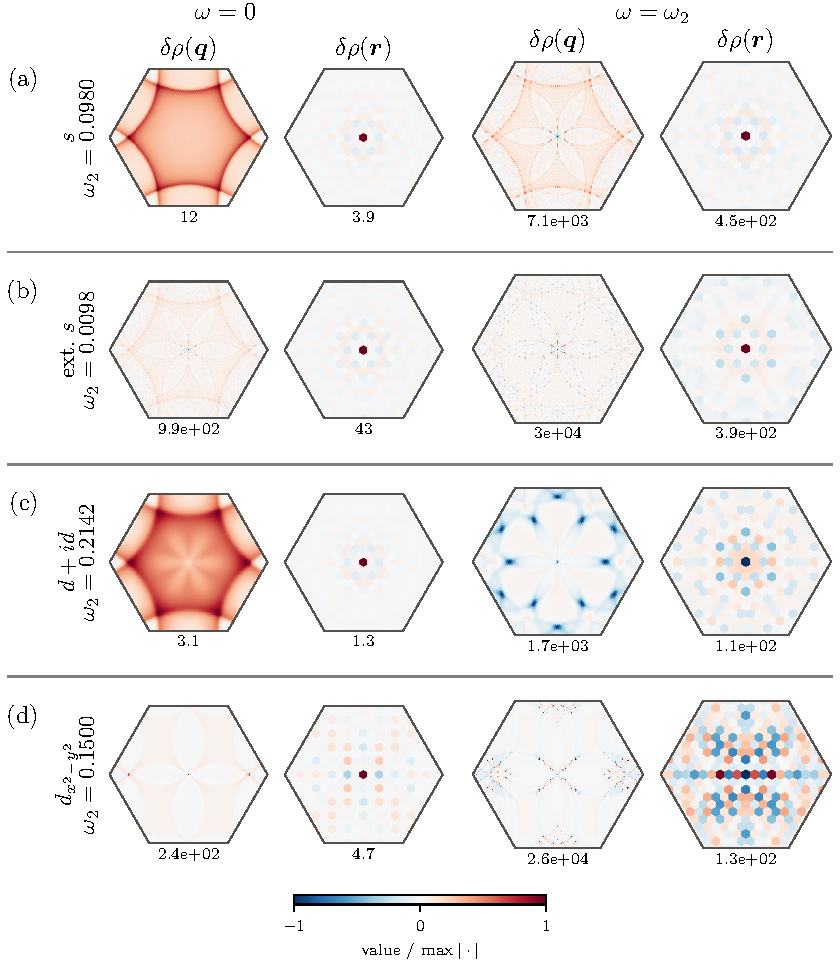
\includegraphics[width=0.85\textwidth]{figs/nosoc_A1imp_all.pdf}
    \caption{No SOC, scalar ($A_1$) impurity, $q_0 = |\bm b_1|$.
    Rows: $s$, extended $s$, $d+id$ and $d_{x^2-y^2}$ pairing.
    Columns: $\operatorname{Re}\delta\rho(\bq)$ and $\delta\rho(\br)$ at $\omega = 0$, then the same at $\omega_2$, which is given on each row.
    The irrep weights of each $\bq$-map are given below it.
    $\operatorname{Im}\delta\rho(\bq)$ and all spin channels vanish.
    Only the nematic $d_{x^2-y^2}$ state has a component beyond $A_1$, from the $E_2$ irrep, which breaks $C_6$ down to $C_2$.}
    \label{fig:nosoc_A1}
\end{figure*}

\paragraph{$A_2$ impurity.}
Next we take an impurity that transforms as $A_2$, i.e.\ odd under the vertical mirrors:
$V(\bk, \bk') = i V_0 (\bk \times \bk')_z \, e^{-|\bk - \bk'|^2/q_0^2}$, with $\hat T = V \tau_z$ and $q_0 = 20 |\bm b_1|$.
For $s$, extended $s$ and $d_{x^2-y^2}$ pairing, $\delta\rho$ vanishes identically at both frequencies.
In these states, $\delta\rho$ is a mirror-even observable, so it cannot couple linearly to a mirror-odd perturbation.
For $d+id$, $\delta\rho$ also vanishes at $\omega = 0$, but it becomes finite near the gap edge (Fig.~\ref{fig:nosoc_A2}).
The response is purely $A_1$, so the product $A_2 \otimes A_2$ appears.
The second $A_2$ factor is the chirality $|\eta_+|^2 - |\eta_-|^2$ of the condensate.
Reversing the chirality should therefore reverse the sign of $\delta\rho$; we have not yet checked this numerically.
An $A_2$ scatterer thus acts as a direct, sign-sensitive probe of chirality, even without SOC.

\begin{figure}[tp]
    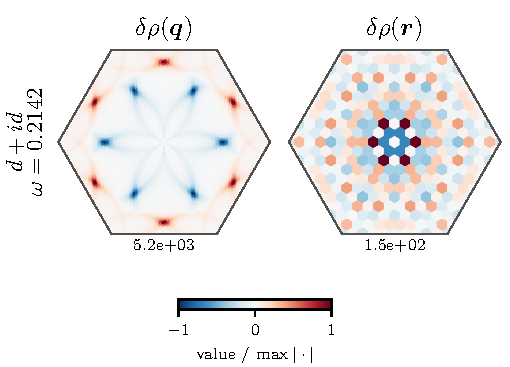
\includegraphics[width=\columnwidth]{figs/nosoc_A2imp_nonzero.pdf}
    \caption{No SOC, $A_2$ impurity, $q_0 = 20|\bm b_1|$: the only non-zero case, $d+id$ at $\omega_2 = 0.2142$, with the panel conventions of Fig.~\ref{fig:nosoc_A1}.
    $\delta\rho$ vanishes identically for $s$, extended $s$ and $d_{x^2-y^2}$ pairing at both frequencies, and for $d+id$ at $\omega = 0$.
    The response is purely $A_1$.}
    \label{fig:nosoc_A2}
\end{figure}

\subsection{Rashba spin-orbit coupling with Ansatz superconducting mean fields}

We add nearest-neighbour Rashba SOC,
$\hat h(\bk) = \varepsilon(\bk) + \alpha\,(\partial_{k_y}\varepsilon\, \sigma_x - \partial_{k_x}\varepsilon\, \sigma_y)$,
with $\alpha = 0.1$ and $\mu = -0.1$.
Pairing is a singlet ansatz, $\hat\Delta = \Psi(\bk)\, i\sigma_y$, with the same four form factors and $|\Delta| = 0.1$.
Figure~\ref{fig:bands} (left) shows the bands for the chiral state.
The impurity is scalar ($A_1$).

The results for the four states are as follows.
\begin{itemize}
    \item $s$, extended $s$, $d_{x^2-y^2}$: only $\delta\rho_0$ is finite (Fig.~\ref{fig:rashba_spin}).
    All spin channels vanish (below $10^{-11}$) at both frequencies.
    $\delta\rho_0$ is $A_1$, with an additional $E_2$ part for $d_{x^2-y^2}$ (weight $15\%$ at $\omega = 0$ and $57\%$ at $\omega = 0.15$; the state is nodal, with four nodes on each helical Fermi surface).
    \item $d+id$ at $\omega = 0$: also only $\delta\rho_0 \in A_1$.
    \item $d+id$ at $\omega = 0.2095$ (gap $0.2137$): all four channels are finite (Fig.~\ref{fig:rashba_spin}).
    $\delta\rho_0$ and $\delta\rho_z$ are real and purely $A_1$.
    $\delta\rho_x(\bq)$ and $\delta\rho_y(\bq)$ are purely imaginary and purely $E_1$.
    They form the vector pattern $\delta\rho_{x,y}(\br) \propto \hat{\bm x}, \hat{\bm y}$, which winds about the impurity.
    In $\bq$-space, the maxima are $|\delta\rho_0| = 1.8\times10^3$, $|\delta\rho_{x}|, |\delta\rho_{y}| \approx 5\times10^2$ and $|\delta\rho_z| = 2.1\times10^2$, so $\delta\rho_z$ is about $12\%$ of $\delta\rho_0$.
\end{itemize}
The out-of-plane spin channel $\delta\rho_z$ is the key signal.
$\sigma_z$ is odd under time reversal and under every vertical mirror.
An $A_1$ pattern in $\delta\rho_z$ is therefore allowed only when both symmetries are broken together, which is exactly the chiral superconducting class.
It is the spin-resolved analogue of the $A_2$-impurity response above.
Here Rashba SOC locks spin to momentum, so a scalar impurity is enough.
The in-plane $E_1$ texture is less specific: in-plane spin $(\sigma_x, \sigma_y)$ already transforms as $E_1$.
In this model it nonetheless appears only in the chiral state.

\begin{figure}[t]
    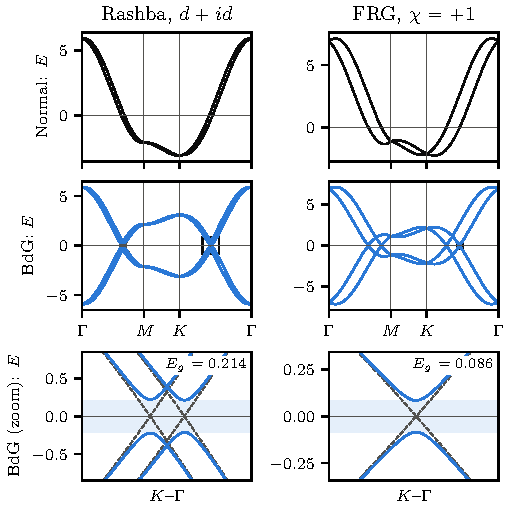
\includegraphics[width=\columnwidth]{figs/bands_combined.pdf}
    \caption{Bands on $\Gamma$--$M$--$K$--$\Gamma$ for the two chiral states.
    Left: Rashba model ($\alpha = 0.1$, $\mu = -0.1$) with $d+id$ singlet pairing, $|\Delta| = 0.1$.
    Right: FRG gap of the Rashba-Hubbard model ($U = 8$, $\alpha = 0.4$, half filling), $\chi = +1$, $\Delta_{\text{rms}} = 0.1$.
    Rows: normal state; BdG bands (solid) with $\pm\varepsilon(\bk)$ (dashed); BdG bands zoomed on the boxed region, the Fermi crossing with the smallest gap on the path.
    The shading marks $|E| < E_g$, with $E_g$ the gap over the whole Brillouin zone.}
    \label{fig:bands}
\end{figure}

\begin{figure*}[tp]
    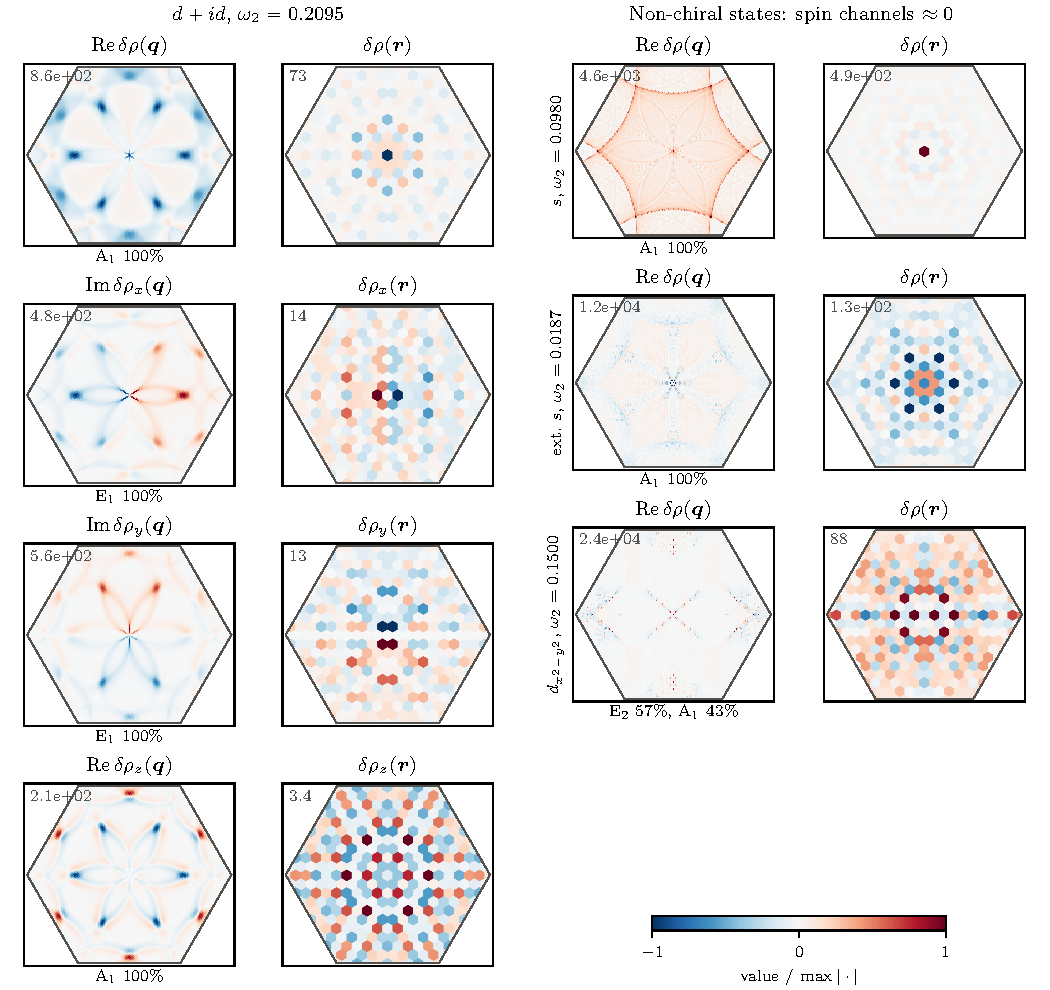
\includegraphics[width=\textwidth]{figs/rashba_spin_all.pdf}
    \caption{Spin-resolved QPI for the Rashba model, scalar impurity, Born approximation, $q_0 = |\bm b_1|$, each state at its $\omega_2$; only non-zero panels are shown.
    Left: $d+id$, rows $\delta\rho_0$, $\delta\rho_x$, $\delta\rho_y$, $\delta\rho_z$; $\delta\rho_z \in A_1$ is finite only in the chiral state.
    Right: $s$, extended $s$ and $d_{x^2-y^2}$, whose spin channels all vanish, so only $\delta\rho_0$ is shown.
    The irrep weights of each $\bq$-map are given below it.
    Each panel is normalised to its own maximum, given in the corner; for the $\bq$-maps this is the maximum over $\bq \neq 0$, so the $\bq = 0$ point saturates.}
    \label{fig:rashba_spin}
\end{figure*}

\subsection{Rashba-Hubbard model with FRG}

We take the superconducting mean field from the leading $\bq = 0$ pairing instability of a divERGe FRG flow for the Rashba-Hubbard model at half filling.
The gap is normalised to $\Delta_{\text{rms}} = 0.1$, and the impurity is again scalar.
\begin{itemize}
    \item $U = 0$, $\alpha = 0.1$: the leading instability is non-degenerate (non-chiral), with gap $0.0777$.
    At $\omega = 0$ and $\omega = 0.0761$, only $\delta\rho_0 \in A_1$ is finite.
    All spin channels vanish.
    \item $U = 8$, $\alpha = 0.4$: the leading instability is two-fold degenerate.
    We take the chiral combination $(v_0 + i v_1)/\sqrt2$, with chirality $\chi = +1$ and gap $0.0863$ (Fig.~\ref{fig:bands}, right).
    The full ansatz pattern appears (Fig.~\ref{fig:frg_spin}).
    $\delta\rho_0, \delta\rho_z \in A_1$ and $\operatorname{Im}\delta\rho_{x,y} \in E_1$, each with weight $1$.
    Unlike the ansatz $d+id$ state, the spin signal is already finite at $\omega = 0$, where $\delta\rho_z$ is about $5\%$ of $\delta\rho_0$ (max $|\delta\rho_z(\bq)| = 0.75$ vs.\ $13.7$).
    At the gap edge ($\omega = 0.0846$), the ratio is also about $5\%$ ($1.7\times10^3$ vs.\ $3.2\times10^4$), while $\delta\rho_{x,y}$ reach about $20\%$.
\end{itemize}
The chirality signature therefore survives in a microscopically derived gap.

\begin{figure}[tp]
    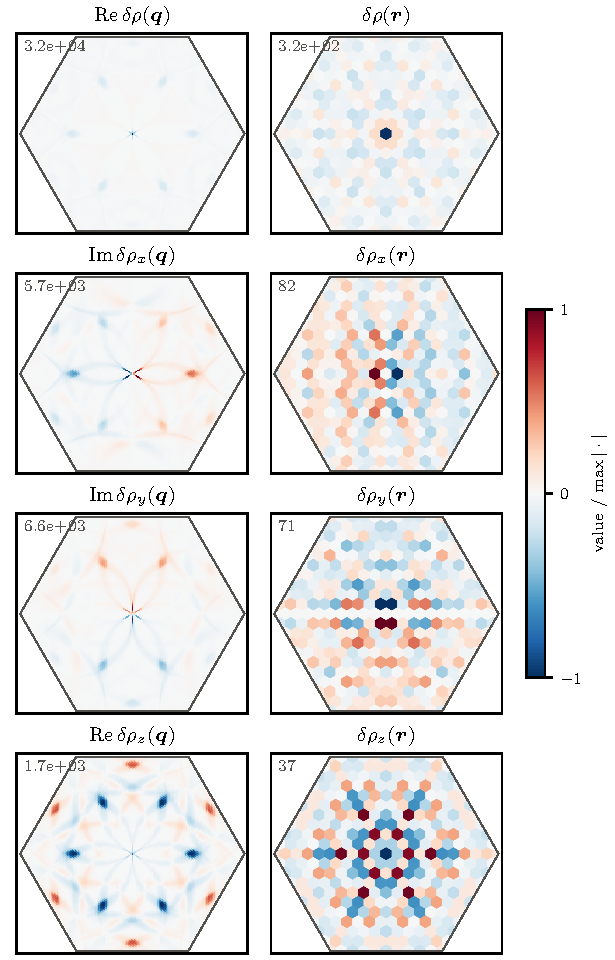
\includegraphics[width=\columnwidth]{figs/frg_spin_chiral.pdf}
    \caption{Spin-resolved QPI for the chiral FRG state of Fig.~\ref{fig:bands}, scalar impurity, $\omega = 0.0846$, $q_0 = |\bm b_1|$.
    Rows: $\delta\rho_0$, $\delta\rho_x$, $\delta\rho_y$, $\delta\rho_z$; $\delta\rho_z$ has an $A_1$ pattern at about $5\%$ of $\delta\rho_0$.}
    \label{fig:frg_spin}
\end{figure}

\subsection{Beyond the Born approximation: full $T$-matrix}
\label{sec:fullT}

For a point-like scalar impurity, the $T$-matrix can be summed to all orders,
$\hat T(\omega) = [1 - \hat V \hat G_{\text{loc}}(\omega)]^{-1} \hat V$, with $\hat V = V_0 \tau_z$ and $\hat G_{\text{loc}}(\omega) = N^{-1} \sum_{\bk} \hat g_0(\bk, \omega)$.
It is independent of $\bq$, so $S(\bq)$, $\delta\rho_\mu$ and the irrep analysis are otherwise unchanged.
A point impurity needs no momentum cutoff, so none is applied in this section ($q_0 \to \infty$).
Born values quoted here for comparison are for the same point impurity; the cutoff is fully symmetric ($A_1$), so it changes amplitudes but never the irreps.
Besides $V_0 = 0.1$, we also use resonant strengths $V_0 = 1/\lambda$, where $\lambda$ is a real eigenvalue of $\hat G_{\text{loc}}(\omega, \Gamma = 0)\, \tau_z$.
At such a $V_0$, the impurity has a bound state at $\omega$, and $\hat T$ is limited only by $\Gamma$.
If all eigenvalues $\lambda$ are complex, there is no bound state at $\omega$.
This is the case for $s$ pairing (Anderson's theorem) and for the non-chiral FRG state.
A bound state needs an energy gap, so resonances are only considered for gapped states, at $\omega$ inside the gap.
They are not considered for the nodal $d_{x^2-y^2}$ state.
Every resonant case is listed in Table~\ref{tab:resonant}.
All other parameters are as above.
At $V_0 = 0.1$, the full $\hat T$ leaves every entry of Table~\ref{tab:cases} unchanged, with or without SOC, except for the Rashba $d+id$ state at $\omega = 0$ discussed below.

\paragraph{Ansatz pairings (Rashba).}
\begin{itemize}
    \item $s$, extended $s$, $d_{x^2-y^2}$: the spin channels still vanish for every $\hat T$, including at resonance.
    $\delta\rho_0$ keeps the irreps it has in the Born approximation.
    For $d_{x^2-y^2}$ this is $A_1$, with an $E_2$ weight of $17\%$ at $\omega = 0$ and $59\%$ at $\omega = 0.15$ for $V_0 = 0.1$.
    The extended-$s$ gap-edge resonances are weak, with $\min|\mathrm{eig}(1 - \hat V \hat G_{\text{loc}})| = 0.19$ and $0.57$.
    The $d_{x^2-y^2}$ state has no gap, so it has no resonances.
    \item $d+id$ at $\omega = 0$: in the Born approximation, only $\delta\rho_0$ is finite.
    With the full $\hat T$, the spin pattern of the gap edge appears here too (Fig.~\ref{fig:fullT_dpid}): $\delta\rho_z \in A_1$ and $\operatorname{Im}\delta\rho_{x,y} \in E_1$, each with weight $1$.
    It is weak at $V_0 = 0.1$, with max $|\delta\rho_z(\bq)| = 2.3\times10^{-3}$ and $|\delta\rho_{x,y}| = 4.1\times10^{-3}$, against $3.7$ for $\delta\rho_0$.
    It is therefore a multiple-scattering effect, absent at first order in $V_0$.
    At the zero-energy resonance, $V_0 = 6.28$ (Fig.~\ref{fig:fullT_dpid_res}), it grows to $\delta\rho_z/\delta\rho_0 \approx 0.4\%$.
    There, $\delta\rho_0$ is dominated by the localised bound state and is almost featureless in $\bq$, while the spin channels keep their $V_0 = 0.1$ patterns.
    \item $d+id$ at $\omega = 0.2095$: the irreps are unchanged.
    At $V_0 = 0.1$, $\delta\rho_z$ grows to $27\%$ of $\delta\rho_0$ ($254$ vs.\ $951$), from $13\%$ in the Born approximation.
    At the two resonances, $V_0 = -2.28$ and $1.33$, $\delta\rho_0$ dominates and the ratio drops to $10^{-4}$ and $1\%$ respectively.
\end{itemize}

\paragraph{FRG pairings.}
\begin{itemize}
    \item $U = 0$, $\alpha = 0.1$: there are no bound states, and only $\delta\rho_0 \in A_1$ is finite, as in the Born approximation.
    \item $U = 8$, $\alpha = 0.4$, chiral ($\chi = +1$): the same irreps as in the Born approximation, each with weight $1$.
    At $\omega = 0$ and $V_0 = 0.1$, $\delta\rho_z/\delta\rho_0 = 5.0\%$, unchanged from Born.
    At the gap edge, the ratio rises from $5.8\%$ to $15\%$ ($2.0\times10^3$ vs.\ $1.3\times10^4$), and $\delta\rho_{x,y}$ reach about $55\%$ of $\delta\rho_0$ (Fig.~\ref{fig:fullT_frg}).
    There are two resonances at $\omega = 0$ ($V_0 = 5.38, 6.56$) and four at the gap edge, compared with one and two for the ansatz $d+id$.
    At these resonances $\delta\rho_z/\delta\rho_0 = 4$--$7\%$ (Table~\ref{tab:resonant}).
\end{itemize}
Going beyond Born therefore never adds an irrep to a channel; it only changes the relative amplitudes.
The chirality signature $\delta\rho_z \in A_1$ survives at all orders.
For the ansatz $d+id$ state, it also extends to $\omega = 0$.

\begin{figure}[tp]
    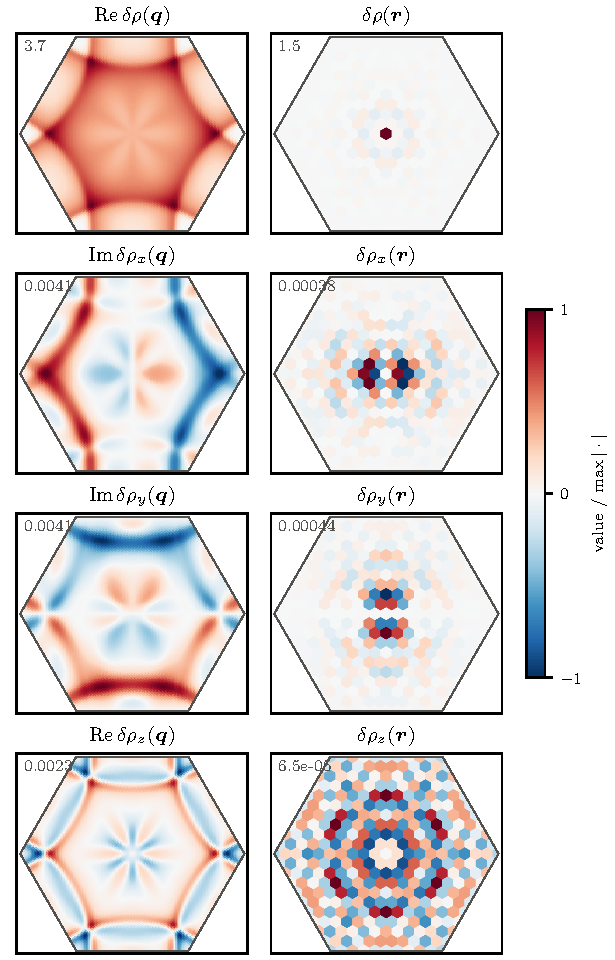
\includegraphics[width=\columnwidth]{figs/fullT_rashba_dpid_om0.pdf}
    \caption{Full $T$-matrix, Rashba model with $d+id$ pairing, scalar impurity, $V_0 = 0.1$, $\omega = 0$.
    Rows: $\delta\rho_0$, $\delta\rho_x$, $\delta\rho_y$, $\delta\rho_z$.
    In the Born approximation only the first row is finite at this frequency.}
    \label{fig:fullT_dpid}
\end{figure}

\begin{figure}[tp]
    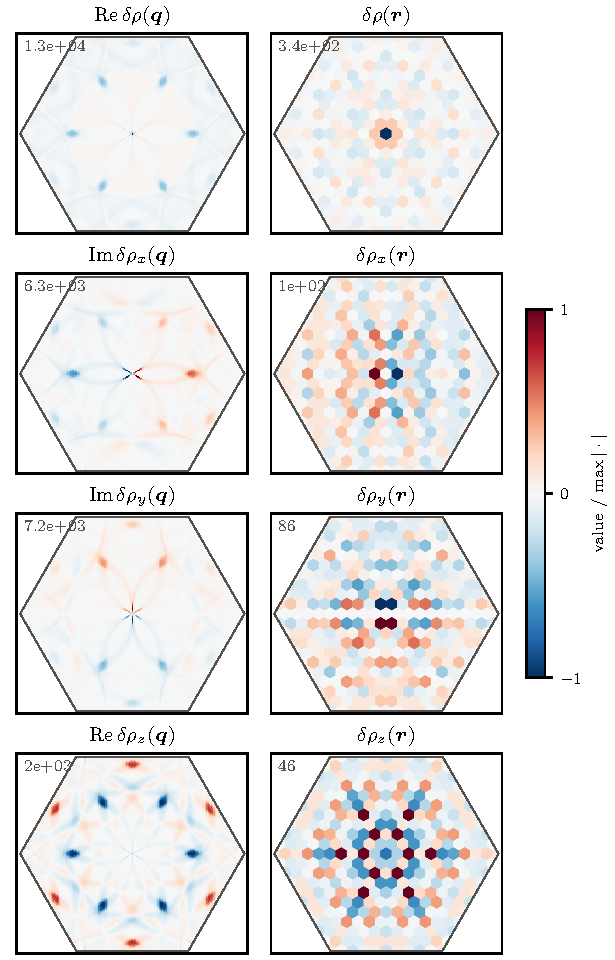
\includegraphics[width=\columnwidth]{figs/fullT_frg_chiral.pdf}
    \caption{Full $T$-matrix for the chiral FRG state of Fig.~\ref{fig:bands}, $V_0 = 0.1$, $\omega = 0.0846$.
    The irreps are those of Fig.~\ref{fig:frg_spin}, but $\delta\rho_z$ is now $15\%$ of $\delta\rho_0$.}
    \label{fig:fullT_frg}
\end{figure}

\begin{figure}[tp]
    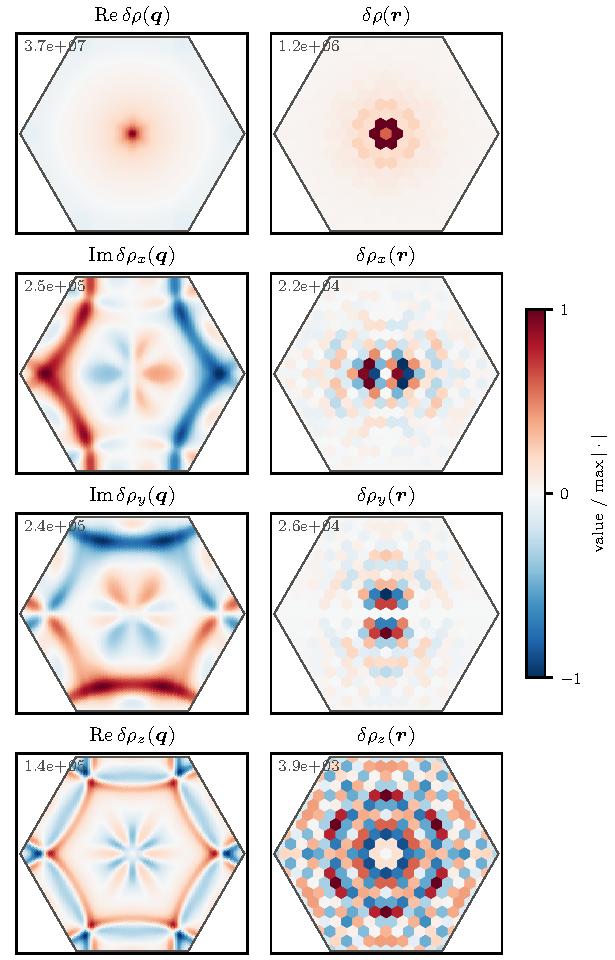
\includegraphics[width=\columnwidth]{figs/fullT_rashba_dpid_om0_res.pdf}
    \caption{As Fig.~\ref{fig:fullT_dpid}, at the zero-energy resonance $V_0 = 6.28$ ($\max|\hat T| = 783$).
    $\delta\rho_0$ becomes a bound-state peak, while $\delta\rho_{x,y} \in E_1$ and $\delta\rho_z \in A_1$ keep the patterns they have at $V_0 = 0.1$.}
    \label{fig:fullT_dpid_res}
\end{figure}

\begin{table*}[tp]
    \caption{Full $T$-matrix at the resonant impurity strengths $V_0 = 1/\lambda$, scalar impurity.
    $\min|\mathrm{eig}|$ is the smallest eigenvalue modulus of $1 - \hat V \hat G_{\text{loc}}(\omega)$ with $\Gamma = 10^{-3}$, which measures how sharp the resonance is.
    Ratios are of the $\bq$-space maxima.
    Where they are finite, $\delta\rho_z \in A_1$ and $\operatorname{Im}\delta\rho_{x,y} \in E_1$, each with weight $1$; $0$ means numerically zero.
    $s$ pairing and the $U = 0$ FRG state have no resonances; the nodal $d_{x^2-y^2}$ state has no gap, so resonances are not considered.}
    \label{tab:resonant}
    \begin{ruledtabular}
    \begin{tabular}{llrrrlrr}
        State & $\omega$ & $V_0$ & $\max|\hat T|$ & $\min|\mathrm{eig}|$ & $\delta\rho_0$ irreps & $\delta\rho_z/\delta\rho_0$ & $\delta\rho_{x,y}/\delta\rho_0$ \\
        \hline
                $d+id$ (Rashba)          & $0.0000$ & $6.28$ & $783$ & $3.7\times10^{-3}$ & $6.7\times10^{-3}$ \\
                                 & $0.2095$ & $-2.28$ & $36.8$ & $1.0\times10^{-4}$ & $2.4\times10^{-4}$ \\
                                 & $0.2095$ & $1.33$ & $40$ & $1.3\times10^{-2}$ & $3.8\times10^{-2}$ \\
        ext.\ $s$ (Rashba)       & $0.0187$ & $-2.96$ & $5.76$ & $0$ & $0$ \\
                                 & $0.0187$ & $1.60$ & $9.29$ & $0$ & $0$ \\
        FRG $U = 8$, $\chi = +1$ & $0.0000$ & $5.38$ & $262$ & $4.0\times10^{-2}$ & $5.6\times10^{-2}$ \\
                                 & $0.0000$ & $6.56$ & $262$ & $4.1\times10^{-2}$ & $5.2\times10^{-2}$ \\
                                 & $0.0846$ & $-1.96$ & $9.54$ & $5.3\times10^{-2}$ & $5.4\times10^{-2}$ \\
                                 & $0.0846$ & $-1.72$ & $8.86$ & $3.7\times10^{-2}$ & $1.5\times10^{-2}$ \\
                                 & $0.0846$ & $1.12$ & $10.9$ & $3.7\times10^{-2}$ & $6.2\times10^{-2}$ \\
                                 & $0.0846$ & $1.22$ & $11.9$ & $7.0\times10^{-2}$ & $6.9\times10^{-2}$ \\
  % from 2026-11-05_fullT/resonant_table.py via note_assets.sh
    \end{tabular}
    \end{ruledtabular}
\end{table*}

\subsection{Sn/Si(111) Wannier model}

% No results yet.

\bibliography{refs}

\end{document}
